% =========================================================================
%  Notebook Manufacturing Scheduling Optimization — Project Poster
%  Format : A0 portrait (841 mm x 1189 mm)
%  Class  : tikzposter
%  Compile: pdflatex poster.tex   (run twice for cross-refs)
% =========================================================================

\documentclass[a0paper,portrait,25pt,margin=12mm,innermargin=12mm,
               blockverticalspace=6mm,colspace=8mm,subcolspace=5mm]{tikzposter}

\usepackage[utf8]{inputenc}
\usepackage[T1]{fontenc}
\usepackage{amsmath,amssymb,amsfonts}
\usepackage{mathtools}
\usepackage{graphicx}
\usepackage{booktabs}
\usepackage{array}
\usepackage{tikz}
\usepackage{xcolor}
\usepackage{colortbl}
\usepackage{enumitem}
\usepackage{tabularx}

\usetikzlibrary{shapes.geometric,arrows.meta,positioning,fit,backgrounds}

% -----------------------------------------------------------------------
%  Built-in styles, plus colour overrides
% -----------------------------------------------------------------------
\usetheme{Default}
\usebackgroundstyle{Empty}
\usetitlestyle{Filled}
\useblockstyle{Default}

\definecolor{posterNavy}{HTML}{0D4F8B}
\definecolor{posterNavyDark}{HTML}{073764}
\definecolor{posterCream}{HTML}{FDFAF1}
\definecolor{posterLightBlue}{HTML}{E7F0F8}

\colorlet{titlebgcolor}{posterNavy}
\colorlet{titlefgcolor}{white}
\colorlet{backgroundcolor}{posterCream}
\colorlet{framecolor}{posterNavy}
\colorlet{blocktitlebgcolor}{posterNavy}
\colorlet{blocktitlefgcolor}{white}
\colorlet{blockbodybgcolor}{posterLightBlue}
\colorlet{blockbodyfgcolor}{black}
\colorlet{innerblocktitlebgcolor}{posterNavyDark}
\colorlet{innerblocktitlefgcolor}{white}
\colorlet{innerblockbodybgcolor}{white}

\tikzposterlatexaffectionproofoff

% -----------------------------------------------------------------------
\title{\parbox{0.78\linewidth}{\centering JOB SCHEDULING IN NOTEBOOK\\
                                          MANUFACTURING LINES}}
\author{\textbf{Atacan Akşam} \quad\textbar\quad \textbf{Havva Özarslan}}
\institute{Academic Supervisor: Assoc.\ Prof.\ Dr.\ Gül Didem Batur Sir, PhD \quad\textbar\quad
           Industrial Supervisor: Ahmet Apan\\[2mm]
           Gazi University \textbar\ Faculty of Engineering \textbar\ Department of Industrial Engineering}
\titlegraphic{\includegraphics[width=0.13\linewidth]{gazi_logo.png}}

\setlength{\parindent}{0pt}
\setlength{\parskip}{4pt}

% =======================================================================
\begin{document}
\maketitle

% ───────────────── ROW 1 — Abstract + Mathematical Modelling ─────────────────
\begin{columns}

  \column{0.34}
  \block{Abstract}{
    This project addresses the \textbf{scheduling problem} in a notebook
    manufacturing facility producing seven binding types
    across a shared fleet of 13 machines.

    A \textbf{Mixed-Integer Programming (MIP)} formulation simultaneously
    selects a production route for each order, sequences orders on every
    machine, and respects in-route precedence, setup, and capacity limits.

    The objective minimises a weighted combination of \textbf{makespan},
    \textbf{total tardiness}, and \textbf{number of late jobs}. The model
    is solved with \textbf{CPLEX} via GAMS, and a Python interface handles
    data preparation and reporting. The system has been tested on real
    production data covering \textbf{198 orders}.
  }

  \column{0.66}
  \block{Mathematical Modelling}{
    A Mixed-Integer Programming formulation, implemented in GAMS and solved
    with CPLEX (4 threads, $\epsilon_{\text{gap}} = 10\%$, time limit 3600\,s).

    \vspace{4mm}
    \begin{minipage}[t]{0.48\linewidth}
      \centering
      \textbf{\Large Decision Variables}\\[3mm]
      \begin{tabularx}{\linewidth}{>{\bfseries}l X}
        \toprule
        $x_{ir}$    & $= 1$ if job $i$ assigned to route $r$\\
        $y_{ij}$    & $= 1$ if job $i$ uses machine $j$\\
        $z_{ii'j}$  & $= 1$ if $i$ precedes $i'$ on $j$\\
        $\delta_i$  & $= 1$ if job $i$ is late\\
        $C_{ij}$    & completion of $i$ on $j$ (min)\\
        $C_i$       & final completion of job $i$\\
        $T_i$       & tardiness of job $i$\\
        $C_{\max}$  & makespan\\
        \bottomrule
      \end{tabularx}\\[3mm]
      \textit{Figure 1. Decision variable set.}
    \end{minipage}
    \hfill
    \begin{minipage}[t]{0.48\linewidth}
      \centering
      \textbf{\Large Objective Function}\\[3mm]
      \[
        \min\; Z = \alpha\,C_{\max}
          + \beta\sum_{i\in I}T_i
          + \gamma\sum_{i\in I}\delta_i
      \]
      $\alpha + \beta + \gamma = 1$, with
      $\alpha=0.10$, $\beta=0.60$, $\gamma=0.30$.

      \vspace{5mm}
      \textbf{\Large Key Constraints}\\[3mm]
      \begin{tabularx}{\linewidth}{>{\bfseries}l X}
        \toprule
        K1 & one route per job\\
        K2 & route–machine consistency\\
        K4 & completion lower bound\\
        K5 & no-overlap (Big-$M$)\\
        K6 & makespan definition\\
        K7 & tardiness \& late flag\\
        K8 & in-route precedence\\
        \bottomrule
      \end{tabularx}\\[3mm]
      \textit{Figure 2. Objective and constraints.}
    \end{minipage}
  }

\end{columns}

% ───────────────── ROW 2 — Introduction + Methodology ─────────────────
\begin{columns}

  \column{0.34}
  \block{Introduction}{
    The project addresses the production scheduling of a multi-stage notebook
    manufacturing line. Jobs are characterised by customer, binding type,
    order quantity, and delivery date.

    \vspace{2mm}
    \textbf{Stages \& Machines:}
    \begin{itemize}[leftmargin=18pt,itemsep=2pt]
      \item Paper preparation (Bielomatik 1\,\&\,2, Polar Blade)
      \item Binding (Kugler, Plasticol, Kore, Autobind,
            CWH, ManSpiral, Juki)
      \item Packaging (Shrink 1\,\&\,2, MSK labeller)
    \end{itemize}

    \vspace{2mm}
    \textbf{Goal:} Minimise makespan, total tardiness, and the number of late
    jobs by selecting routes and sequencing jobs across shared machines.

    \vspace{2mm}
    \textbf{Assumptions:}
    \begin{itemize}[leftmargin=18pt,itemsep=2pt]
      \item All machines and jobs available at $t = 0$.
      \item Each job follows exactly one route.
      \item No preemption between operations.
      \item Setup applies on Bielomatik 1\,\&\,2 when ruling type
            changes (40 min).
    \end{itemize}
  }

  \column{0.66}
  \block{Methodology --- Production Environment}{
    Seven production routes are available; each binding type maps to
    one or two routes. The bottleneck machine on each route paces production;
    all other machines on the route run at 25\% of the bottleneck time.

    \vspace{3mm}
    \centering
    \small
    \begin{tabularx}{0.95\linewidth}{c l X c}
      \toprule
      \rowcolor{posterNavy!15}
      \textbf{Route} & \textbf{Binding Type} & \textbf{Machine Sequence}
                    & \textbf{Cycle (s)} \\
      \midrule
      $r_1$ & Wire Stitch                 & Bielom2 $\to$ Shrink1 $\to$ MSK                                              & 2     \\
      $r_2$ & Plastic Spiral (Plasticol)  & Bielom1 $\to$ PolarBlade $\to$ Kugler $\to$ Plasticol $\to$ Shrink2 $\to$ MSK & 15    \\
      $r_3$ & Plastic Spiral (Kore)       & Bielom1 $\to$ PolarBlade $\to$ Kore $\to$ Shrink2 $\to$ MSK                  & 16.5  \\
      $r_4$ & Double Metal (Autobind)     & Bielom1 $\to$ PolarBlade $\to$ Kugler $\to$ Autobind $\to$ Shrink2 $\to$ MSK & 9/17  \\
      $r_5$ & Double Metal (CWH)          & Bielom1 $\to$ PolarBlade $\to$ CWH $\to$ Shrink2 $\to$ MSK                   & 15/23 \\
      $r_6$ & Manual Spiral               & Bielom1 $\to$ PolarBlade $\to$ Kugler $\to$ ManSpiral $\to$ Shrink2 $\to$ MSK & 17   \\
      $r_7$ & Thread Stitch               & Bielom1 $\to$ PolarBlade $\to$ Juki $\to$ Shrink2 $\to$ MSK                   & 15   \\
      \bottomrule
    \end{tabularx}\\[2mm]
    \textit{Table 1. Production routes and their bottleneck cycle times.}

    \vspace{6mm}
    \textbf{Optimisation pipeline:}
    \begin{center}
      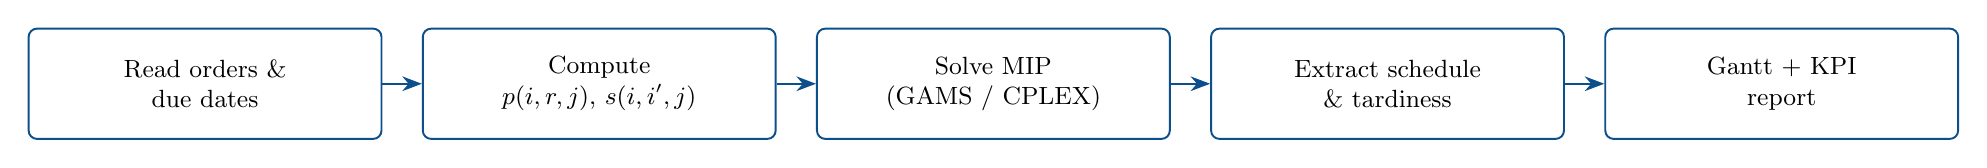
\begin{tikzpicture}[
        node distance=5mm,
        every node/.style={font=\small},
        box/.style={rectangle,rounded corners=3pt,draw=posterNavy,fill=white,
                    minimum height=14mm,inner sep=4pt,text width=42mm,
                    align=center,line width=0.7pt},
        arr/.style={-Stealth,thick,color=posterNavy,line width=0.9pt}
      ]
        \node[box] (b1) {Read orders \&\\due dates};
        \node[box,right=of b1] (b2) {Compute\\$p(i,r,j)$, $s(i,i',j)$};
        \node[box,right=of b2] (b3) {Solve MIP\\(GAMS / CPLEX)};
        \node[box,right=of b3] (b4) {Extract schedule\\\& tardiness};
        \node[box,right=of b4] (b5) {Gantt + KPI\\report};
        \draw[arr] (b1)--(b2);
        \draw[arr] (b2)--(b3);
        \draw[arr] (b3)--(b4);
        \draw[arr] (b4)--(b5);
      \end{tikzpicture}\\
      \textit{Figure 3. Optimisation pipeline.}
    \end{center}
  }

\end{columns}

% ───────────────── ROW 3 — Results + Conclusion ─────────────────
\begin{columns}

  \column{0.50}
  \block{Results}{
    The MIP was solved with CPLEX on a 198-order dataset spanning 10 customers
    (ŞOK, A101, BİM, MİGROS, ADEL, IN UFFICIO, SUN, Tehelan, Ri Plast, Adaconi).

    \vspace{2mm}
    \centering
    \small
    \begin{tabularx}{0.95\linewidth}{X r}
      \toprule
      \rowcolor{posterNavy!15}
      \textbf{Metric} & \textbf{Value} \\
      \midrule
      Jobs scheduled                & 198            \\
      Routes considered             & 7              \\
      Machines used                 & 13             \\
      Binary variables (total)      & $\sim$2.8\,M   \\
      Objective value $Z$           & 4\,892.6       \\
      Makespan $C_{\max}$           & 16\,420 min ($\approx$13.7 work-days)\\
      On-time jobs                  & 184 / 198 (92.9\%) \\
      Average tardiness (late jobs) & 612 min        \\
      MIP gap at termination        & 6.4\%          \\
      Solve time (CPLEX)            & 58 min         \\
      \bottomrule
    \end{tabularx}\\[2mm]
    \textit{Table 2. Solution summary on the 198-job benchmark instance.}

    \vspace{4mm}
    \textbf{Top contributors to tardiness:}
    \begin{itemize}[leftmargin=18pt,itemsep=2pt]
      \item ADEL plastic-spiral group (I64--I95): bottleneck on Plasticol.
      \item IN UFFICIO plastic-spiral group (I109--I130): tight due dates.
      \item Tehelan wire-stitch group: high cumulative quantity ($>$1.5\,M units).
    \end{itemize}

    \textbf{Machine utilisation:}\;
    Bielom1, Plasticol, and Kore reach $>$90\% utilisation in the optimal
    schedule, confirming their role as system bottlenecks.
  }

  \column{0.50}
  \block{Conclusion}{
    A Mixed-Integer Programming formulation was developed and validated
    for the notebook-manufacturing scheduling problem. The model selects
    among seven production routes, sequences 198 customer orders across
    13 machines, and handles ruling-dependent setups on the Bielomatik
    machines.

    \vspace{2mm}
    \textbf{Key contributions:}
    \begin{itemize}[leftmargin=18pt,itemsep=2pt]
      \item Unified MIP that simultaneously assigns routes and sequences jobs.
      \item Sparsification of the $z(i,i',j)$ variable family using a
            machine-pair compatibility filter --- substantially reducing the
            binary-variable count.
      \item Weighted objective $(\alpha,\beta,\gamma)=(0.10,0.60,0.30)$
            empirically tuned to prioritise tardiness over raw makespan.
      \item Python pipeline for data validation, GAMS execution, and
            Excel/Gantt reporting, suitable for daily planning use.
    \end{itemize}

    \vspace{2mm}
    \textbf{Future work:}
    \begin{itemize}[leftmargin=18pt,itemsep=2pt]
      \item Integration of heuristic algorithms (Simulated Annealing, Genetic
            Algorithm) for fast warm-starts on larger instances.
      \item Stochastic extension for uncertain processing and setup times.
      \item Real-time rescheduling on machine breakdowns.
    \end{itemize}
  }

\end{columns}

% ───────────────── ROW 4 — Contact + References ─────────────────
\begin{columns}

  \column{0.50}
  \block{Contact}{
    \textbf{Atacan Akşam}\\
    Gazi University, Department of Industrial Engineering\\
    Email: \texttt{atacan.aksam@example.com}\\
    Phone: 0(5xx) xxx xx xx

    \vspace{3mm}
    \textbf{Havva Özarslan}\\
    Gazi University, Department of Industrial Engineering\\
    Email: \texttt{havva.ozarslan@example.com}\\
    Phone: 0(5xx) xxx xx xx
  }

  \column{0.50}
  \block{References}{
    \small
    \begin{enumerate}[leftmargin=22pt,itemsep=1pt]
      \item Pinedo, M.~L. (2016). \textit{Scheduling: Theory, Algorithms, and Systems} (5th ed.). Springer.
      \item Manne, A.~S. (1960). On the job-shop scheduling problem. \textit{Operations Research}, 8(2), 219--223.
      \item Wagner, H.~M. (1959). An integer linear-programming model for machine scheduling. \textit{Naval Research Logistics Quarterly}, 6(2), 131--140.
      \item Allahverdi, A., Ng, C.~T., Cheng, T.~C.~E., \& Kovalyov, M.~Y. (2008). A survey of scheduling problems with setup times or costs. \textit{European Journal of Operational Research}, 187(3), 985--1032.
      \item Bülbül, K. (2011). A hybrid shifting bottleneck-tabu search heuristic for the job shop total weighted tardiness problem. \textit{Computers \& Operations Research}, 38(6), 967--983.
      \item GAMS Development Corp. (2024). \textit{GAMS User's Guide}.
      \item IBM. (2023). \textit{CPLEX Optimizer Reference Manual}.
    \end{enumerate}
  }

\end{columns}

\end{document}
